\usetikzlibrary{arrows,positioning}

\subsection{Configurators in the Wild}

\subsubsection*{Notebooks}

\begin{frame}{\myframetitle}
	\begin{mycolumns}[widths={70,30}]
		\myexampletight{Configuring a Notebook}{
			\only<1,3->{\pic[width=\linewidth]{thinkpad-x1-yoga-display}}\only<2|handout:0>{\pic[width=\linewidth]{thinkpad-x1-yoga-display-invalidconf}}
		}
	\mynextcolumn
		\mynote{}{
			can detect mistakes, but provides no explanations or fixes
		}
	\end{mycolumns}
\end{frame}

\begin{frame}{\myframetitle}
	\begin{mycolumns}[widths={70,30}]
		\myexampletight{Still Configuring a Notebook}{
			\pic[width=\linewidth]{thinkpad-x1-yoga-office}
		}
	\mynextcolumn
		\mynote{}{
			allows some feature combinations and not others, prices are opaque
		}
	\end{mycolumns}
\end{frame}

\subsubsection*{Cars}

\begin{frame}{\myframetitle}
	\begin{mycolumns}[widths={40,60},animation=none]
	\mynextcolumn
		\myexampletight{Configuring a Car}{
			\pic[width=\linewidth]{toyota-aygo-wheels}
		}
	\end{mycolumns}
\end{frame}

\begin{frame}{\myframetitle}
	\begin{mycolumns}[widths={40,60},reverse]
		\mynote{}{
			it is possible to create inconsistent states, leading to an invalid product
		}
	\mynextcolumn
		\myexampletight{Configuring a Car with a Weird Price}{
			\centering\pic[width=.55\linewidth]{toyota-aygo-costs}
		}
	\end{mycolumns}
\end{frame}

\begin{frame}{\myframetitle}
	\begin{mycolumns}[widths={40,60},reverse]
		\mynote{}{
			What happens if we ordered this \ldots?
		}
	\mynextcolumn
		\myexampletight{Configuring a Car with 8 Wheels!}{
			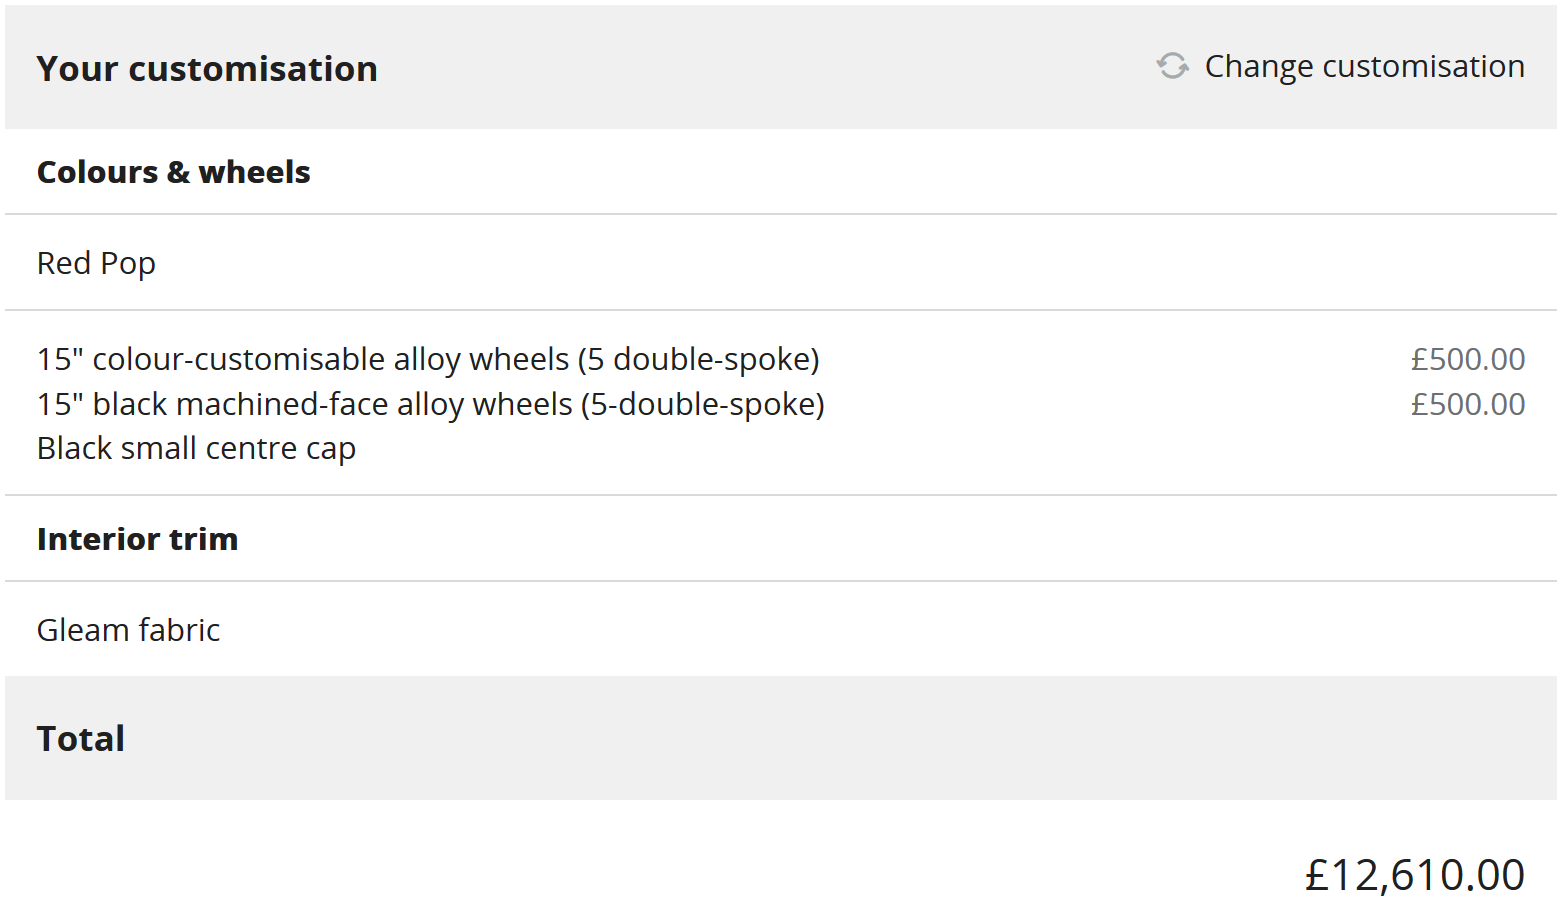
\includegraphics[width=\linewidth]{toyota-aygo-costs3}
		}
	\end{mycolumns}
\end{frame}

\begin{frame}{\myframetitle}
	\begin{mycolumns}[widths={70,30}]
		\myexampletight{Configuring a German Car}{
			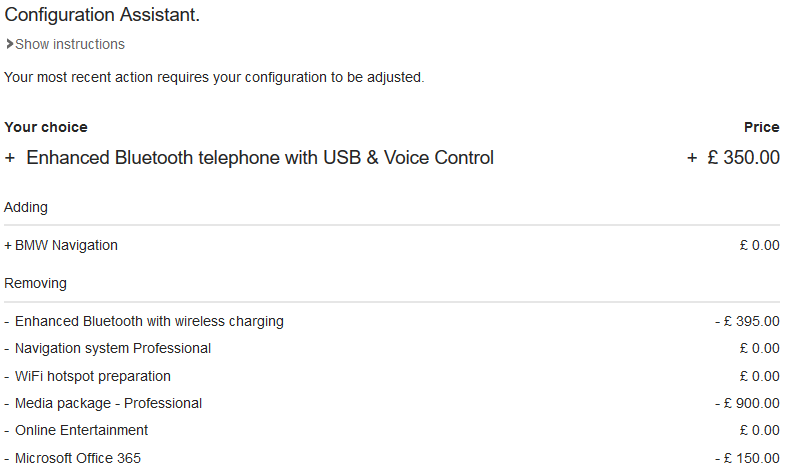
\includegraphics[width=\linewidth]{bmw-series1-confassistant-bluetooth}
		}
	\mynextcolumn
		\mynote{}{
			Why does the telephone conflict with Microsoft Office?
		}
	\end{mycolumns}
\end{frame}

\subsubsection*{Linux Kernel}

\begin{frame}{\myframetitle}
	\begin{mycolumns}[widths={60,40}]
		\myexampletight{}{
			\pic[width=\textwidth]{linux-menuconfig} % sudo apt install make flex bison libncurses5-dev && make menuconfig
		}
	\mynextcolumn
		\mynote{make menuconfig}{
			\begin{itemize}
				\item configures KConfig models
				\item generates a \texttt{.config} file
				\item widely used to configure Linux
				\item still: it is possible to create invalid products
			\end{itemize}
		}
	\end{mycolumns}
\end{frame}

\subsection{Automated Analysis of Feature Models}

\begin{frame}{\myframetitle}
	\begin{mycolumns}
		\mynote{Open Questions}{
			\begin{itemize}
				\item How do such configurators work?
				\item How to avoid inconsistencies?
				\item How to provide explanations and fixes?
    			\item How to get all valid configurations automatically? (\emph{P2(b)})
			\end{itemize}
		}
		\mydefinition{Automated Analysis of Feature Models}{
			\begin{itemize}
				\item up until now: \emph{creation} and \emph{transformation} of feature models
				\item now: \emph{analysis} of feature models to improve our understanding of a configuration space
				\item for brevity: product = valid configuration
			\end{itemize}
		}
	\mynextcolumn
		\myexample{Asking Questions About Feature Models}{
			\begin{itemize}
				\item Is a given configuration valid?
				\item Is there any product at all?\\
					How many/which products are there?\\
				\item Is a given feature (de-)selectable at all?\\
					How many/which products include it?\\
				\item Is a given partial configuration consistent?\\
					How many/which products include it?\\
				\item \color{gray}{(Which features always occur together?)}
				\item \color{gray}{(Is a given constraint redundant?)}
				\item \color{gray}{(How do two feature model versions differ?)}
				\item \color{gray}{(Why is \ldots? How to fix \ldots?)}
			\end{itemize}
		}
	\end{mycolumns}
\end{frame}

\subsection{SAT, \ssat{}, and AllSAT Solvers}

\begin{frame}{\myframetitle}
	\begin{mycolumns}
		\mydefinition{Recap: Boolean Satisfiability Problem (SAT)}{
			\begin{itemize}
				\item \emph{decision problem}: is there any assignment that satisfies a given formula?
				\item formally: $SAT(\phi) \mequals \exists A \colon \phi(A) = \top$
				\item known to be \emph{NP-complete}:\\
					in theory, difficult to solve if $P \neq NP$;\\
					in practice, solvability depends on domain
				\item answered by \emph{SAT solvers}:\\
					highly-optimized, off-the-shelf tools;\\
					competitively developed over several decades;\\
					takes a CNF in DIMACS format as input
			\end{itemize}
		}
		\myexample{}{
			\begin{itemize}
				\item $X \pimplies Y$ is satisfiable
				\item $X \por \pnot X$ is satisfiable (even tautological)
				\item $X \pand \pnot X$ is not satisfiable (why?)
			\end{itemize}
		}
	\mynextcolumn
		\mydefinition{Sharp Satisfiability Problem (\ssat{})}{
			\begin{itemize}
				\item \emph{counting problem}: how many assignments satisfy a given formula?
				\item $\ssat(\phi) = \abs{\{A \mid \phi(A) = \top\}}$
				\item known to be \emph{\texttt{\#}P-complete}:\\
					at least as hard as SAT (probably harder)
				\item answered by \emph{\ssat{} solvers}
			\end{itemize}
		}
		\mydefinition{Solution Enumeration Problem (AllSAT)}{
			\begin{itemize}
				\item \emph{enumeration problem}: which assignments satisfy a given formula?
				\item $AllSAT(\phi) = \{A \mid \phi(A) = \top\}$
				\item at least as hard as \ssat{} (probably harder)
				\item answered by \emph{AllSAT solvers}
			\end{itemize}
		}
	\end{mycolumns}
\end{frame}

\begin{frame}{Automated Analysis of Feature Models}
	\begin{mycolumns}
		\myexample{Asking Questions About Feature Models}{
			\begin{itemize}
				\item Is a given configuration valid? $\Rightarrow$ \emph{evaluate}
				\item \emph{Is} there any valid configuration at all?\\
					\emph{How many}/\emph{which} valid configurations are there?\\
				\item \emph{Is} a given feature (de-)selectable at all?\\
					\emph{How many}/\emph{which} valid configurations include it?\\
				\item \emph{Is} a given partial configuration consistent?\\
					\emph{How many}/\emph{which} valid configurations include it?\\
			\end{itemize}
		}
		\mynote{Choosing the Right Solver}{
			\begin{itemize}
				\item ``is?''~~~~~~~~~~~~$\approx$ SAT solver query
				\item ``how many?''~$\approx$ \ssat{} solver query
				\item ``which?''~~~~~~\,$\approx$ AllSAT solver query
			\end{itemize}
		}
	\mynextcolumn
		\mydefinition{Typical Feature-Model Analysis Process}{
			\centering
			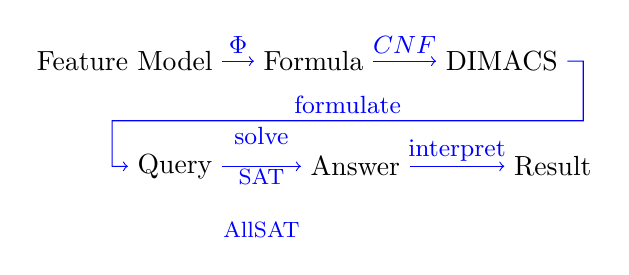
\begin{tikzpicture}
				\tikzset{block/.style={align=center,minimum height=5mm}}
				\node [block] (fm) {Feature Model};
				\node [block, right =4mm of fm] (formula) {Formula};
				\node [block, right =8mm of formula] (cnf) {DIMACS};
				\node [block, below right =8mm and -12mm of fm] (query) {Query};
				\node [block, right =10mm of query] (answer) {Answer};
				\node [block, right =12mm of answer] (result) {Result};
				\node [coordinate, below right =5mm and 2mm of cnf] (right) {};
				\node [coordinate, above left =3mm and 2mm of query] (left) {};
				\path[draw,->,color=blue] (fm) edge node[yshift=2mm] {\small $\Phi$} (formula)
							(formula) edge node[yshift=2mm] {\small $CNF$} (cnf)
							(cnf.east) -| (right) -- node[yshift=2mm] {\small formulate} (left) |- (query)
							(query) edge node[yshift=-2mm,align=center,font={\footnotesize}] {{\small solve}\\[1.5ex]SAT\\\ssat{}\\AllSAT} (answer)
							(answer) edge node [yshift=2mm]{\small interpret} (result);
			\end{tikzpicture}
		}
		\mynote{}{
			for brevity, we assume that $\phi = CNF(\Phi(FM))$ for a given feature model $FM$
		}
	\end{mycolumns}
\end{frame}

\subsection{Consistency, Cardinality, and Enumeration Queries}

\subsubsection{Feature Model}

\begin{frame}{\myframetitle}
	\begin{mycolumns}[t]
		\emph{Consistency of Feature Models (SAT)}
		\mydefinition{Void/Consistent Feature Model}{
			\begin{itemize}
				\item are there grave modeling errors?
				\item is it possible to configure any product at all?
			\end{itemize}
			\centering
			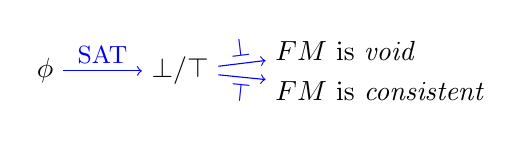
\begin{tikzpicture}
				\tikzset{block/.style={align=center,minimum height=5mm}}
				\node [block] (query) {$\phi$};
				\node [block, right =10mm of query] (answer) {$\bot/\top$};
				\node [block, above right =-3mm and 6mm of answer] (void) {$FM$ is \emph{void}};
				\node [block, below right =-3mm and 6mm of answer] (notvoid) {$FM$ is \emph{consistent}};
				\path[draw,->,color=blue] (query) edge node[yshift=2mm] {\small SAT} (answer)
							(answer) edge node [yshift=2mm,sloped]{\small $\bot$} (void)
							(answer) edge node [yshift=-2mm,sloped]{\small $\top$} (notvoid);
			\end{tikzpicture}
		}
		\mynextcolumn
		\emph{Cardinality of Feature Models (\ssat{})}
		\mydefinition{How Many Products Are There?}{
			\centering
			\begin{tikzpicture}
				\tikzset{block/.style={align=center,minimum height=5mm}}
				\node [block] (query) {$\phi$};
				\node [block, right =10mm of query] (answer) {$\abs{C}$};
				\path[draw,->,color=blue] (query) edge node[yshift=2mm] {\small \ssat{}} (answer);
			\end{tikzpicture}
		}
		\mydefinition{Variability Factor: Share of Products?}{
			\centering
			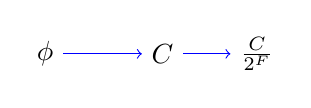
\begin{tikzpicture}
				\tikzset{block/.style={align=center,minimum height=5mm}}
				\node [block] (query) {$\phi$};
				\node [block, right =10mm of query] (answer) {$\abs{C}$};
				\node [block, right =6mm of answer] (num) {$\frac{\abs{C}}{2^{\abs{F}}}$};
				\path[draw,->,color=blue] (query) edge node[yshift=2mm] {\small \ssat{}} (answer)
							(answer) edge node [yshift=2mm,sloped]{} (num);
			\end{tikzpicture}
		}
	\end{mycolumns}
	\begin{mycolumns}[t]
		\myexampletight{}{
			\leftandright{
				\centering
				{\small\featureDiagram{Root,concrete[X,concrete,alternative][Y,concrete]}\\$\pnot (X \por Y)$}

				void
			}{
				\centering
				{\small\featureDiagram{Root,concrete[X,concrete,alternative][Y,concrete]}\\$X \por Y$}

				consistent
			}
		}
		\mynextcolumn
		\myexampletight{}{
			\leftandright{
				\centering
				{\small\featureDiagram{Root,concrete[X,concrete,alternative][Y,concrete]}\\$\pnot (X \por Y)$}

				$0$ products, VF $0$
			}{
				\centering
				{\small\featureDiagram{Root,concrete[X,concrete,alternative][Y,concrete]}\\$X \por Y$}

				$2$ products, VF $\frac{2}{8}$
			}
		}
	\end{mycolumns}
\end{frame}

\begin{frame}{\myframetitle}
	\begin{mycolumns}[t]
		\emph{Feasibility of SAT-Based Analyses}

		\mynote{Is SAT-Based Analysis ``Easy''?}{
			\begin{itemize}
				\item provocative claim: \mycite{SAT-based analysis of feature models is easy} \mysource{\href{https://dl.acm.org/doi/10.5555/1753235.1753267}{Mendonca~et~al.~2009}}
				\item easy $=$ performs much better than expected (although NP-complete)
				\item easy $=$ fast?
				\begin{itemize}
					\item what about formulating the query?\\
						(e.g., CNF transformation)
					\item what about many queries?\\
						(e.g., what we discuss next)
				\end{itemize}
			\end{itemize}
		}
	\mynextcolumn
		\emph{Feasibility of \ssat{}-Based Analyses}
	
		\myexampletight{Time to Count Products of Linux}{
			\includegraphics[width=\linewidth,page=4]{linux-plots}
		}
	\end{mycolumns}
\end{frame}


\begin{frame}{\myframetitle}
	\begin{mycolumns}
		\emph{Enumeration of Feature Models (AllSAT)}
		\mydefinition{Which Products Are There?}{
			\begin{itemize}
				\item \emph{P2(b)}: How to get all products?
			\end{itemize}
			\centering
			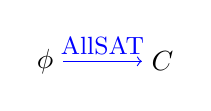
\begin{tikzpicture}
				\tikzset{block/.style={align=center,minimum height=5mm}}
				\node [block] (query) {$\phi$};
				\node [block, right =10mm of query] (answer) {$C$};
				\path[draw,->,color=blue] (query) edge node[yshift=2mm] {\small AllSAT} (answer);
			\end{tikzpicture}
		}
		\mynote{}{
			AllSAT does not scale to realistic feature models!\\
			50 features, configurations \`a 1 Byte $\approx$ 1 Petabyte
		}
		\myexampletight{}{
			\leftandright{
				\centering
				{\small\featureDiagram{Root,concrete[X,concrete,alternative][Y,concrete]}\\$\pnot (X \por Y)$}

				$\varnothing$
			}{
				\centering
				{\small\featureDiagram{Root,concrete[X,concrete,alternative][Y,concrete]}\\$X \por Y$}

				$\{\{Root, X\},\{Root, Y\}\}$
			}
		}
	\mynextcolumn
		\centering
		\sffamily
		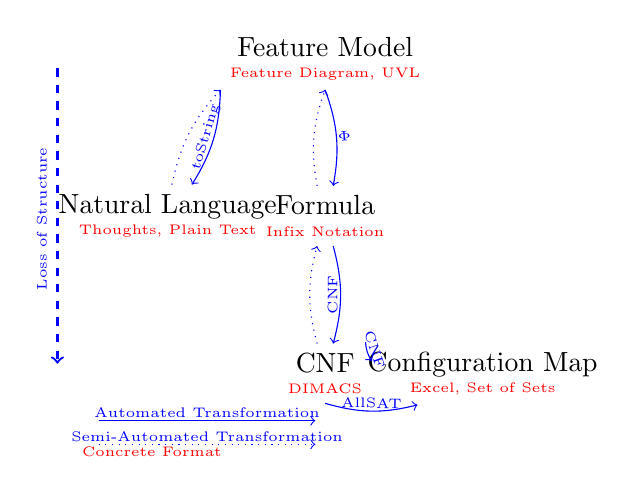
\begin{tikzpicture}
			\tikzstyle{every edge}=[font=\tiny,draw,color=blue]

			\node (topleft) at (-1.4,0) {};
			\node (bottomleft) at (-1.4,-4) {};
			
			\node (fd) at (2,0) [align=center] {Feature Model\\[-1ex]{\tiny\color{red}Feature Diagram, UVL}};
			\node (nat) at (0,-2) [align=center] {Natural Language\\[-1ex]{\tiny\color{red}Thoughts, Plain Text}};
			\node (phi) at (2,-2) [align=center] {Formula\\[-1ex]{\tiny\color{red}Infix Notation}};
			\node (cfg) at (4,-4) [align=center] {Configuration Map\\[-1ex]{\tiny\color{red}Excel, Set of Sets}};
			\node (cnf) at (2,-4) [align=center] {CNF\\[-1ex]{\tiny\color{red}DIMACS}};

			\path [dashed, thick, ->] (topleft) edge node[left, rotate=90, yshift=2mm, xshift=10mm] {Loss of Structure} (bottomleft);
		
			\path [->] (fd.south west) edge[bend left=15] node[sloped,yshift=1mm] {toString} (nat);
			\path [dotted, ->] (nat) edge[bend left=15] node[sloped,yshift=1mm] {} (fd.south west);
			
			\path [->] (fd.south) edge[bend left=15] node[sloped,yshift=1mm,rotate=90] {$\Phi$} (phi);
			\path [dotted, ->] (phi) edge[bend left=15] node[sloped,yshift=2mm,rotate=270] {} (fd.south);

			\path [->] (phi) edge[bend left=15] node[sloped,yshift=1mm] {CNF} (cnf);
			\path [dotted, ->] (cnf) edge[bend left=15] node[sloped,yshift=2mm,rotate=270] {} (phi);
		
			\path [->] (cfg) edge[bend right=15] node[sloped,yshift=1mm] {CNF} (cnf);
			\path [->] (cnf.south) edge[bend right=15] node[sloped,yshift=1mm] {AllSAT} (cfg);

			\node (trans) at (-1,-4.6) {};
			\node (trans2) at (2,-4.6) {};
			\node (trans3) at (-1,-4.9) {};
			\node (trans4) at (2,-4.9) {};
			\path [->] (trans) edge node[yshift=1mm] {Automated Transformation} (trans2);
			\path [dotted, ->] (trans3) edge[yshift=5mm] node[yshift=1mm] {Semi-Automated Transformation} (trans4);
		
			\node (bottomleft2) at (-0.2,-5) {\tiny\color{red}Concrete Format};
		\end{tikzpicture}
	\end{mycolumns}
\end{frame}

\subsubsection{Features}

\begin{frame}{\myframetitle}
	\begin{mycolumns}[t]
		\emph{Consistency of Features (SAT)}
		\mydefinition{Core/Dead Feature}{
			\begin{itemize}
				\item can a feature $F$ be (de-)selected at all?
			\end{itemize}
			\centering
			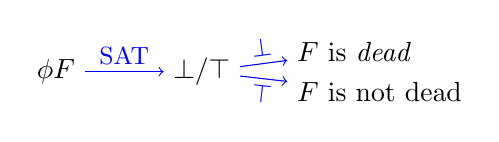
\begin{tikzpicture}
				\tikzset{block/.style={align=center,minimum height=5mm}}
				\node [block] (query) {$\phi \pand F$};
				\node [block, right =10mm of query] (answer) {$\bot/\top$};
				\node [block, above right =-3mm and 6mm of answer] (void) {$F$ is \emph{dead}};
				\node [block, below right =-3mm and 6mm of answer] (notvoid) {$F$ is not dead};
				\path[draw,->,color=blue] (query) edge node[yshift=2mm] {\small SAT} (answer)
							(answer) edge node [yshift=2mm,sloped]{\small $\bot$} (void)
							(answer) edge node [yshift=-2mm,sloped]{\small $\top$} (notvoid);
			\end{tikzpicture}
			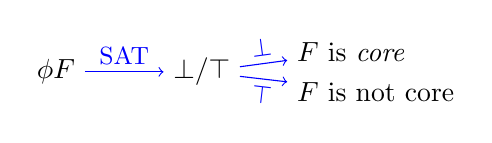
\begin{tikzpicture}
				\tikzset{block/.style={align=center,minimum height=5mm}}
				\node [block] (query) {$\phi \pand \pnot F$};
				\node [block, right =10mm of query] (answer) {$\bot/\top$};
				\node [block, above right =-3mm and 6mm of answer] (void) {$F$ is \emph{core}};
				\node [block, below right =-3mm and 6mm of answer] (notvoid) {$F$ is not core};
				\path[draw,->,color=blue] (query) edge node[yshift=2mm] {\small SAT} (answer)
							(answer) edge node [yshift=2mm,sloped]{\small $\bot$} (void)
							(answer) edge node [yshift=-2mm,sloped]{\small $\top$} (notvoid);
			\end{tikzpicture}
		}
		\mynextcolumn
		\emph{Cardinality of Features (\ssat{})}
		\mydefinition{How Many Products Include Feature $F$?}{
			\centering
			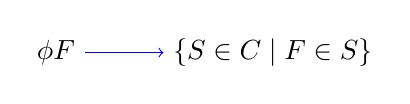
\begin{tikzpicture}
				\tikzset{block/.style={align=center,minimum height=5mm}}
				\node [block] (query) {$\phi \pand F$};
				\node [block, right =10mm of query] (answer) {$\abs{\{S \in C \mid F \in S\}}$};
				\path[draw,->,color=blue] (query) edge node[yshift=2mm] {\small \ssat{}} (answer);
			\end{tikzpicture}
		}
		\mydefinition{Commonality: How Dead is This Feature?}{
			\centering
			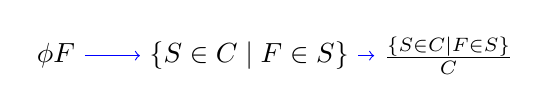
\begin{tikzpicture}
				\tikzset{block/.style={align=center,minimum height=5mm}}
				\node [block] (query) {$\phi \pand F$};
				\node [block, right =7mm of query] (answer) {$\abs{\{S \in C \mid F \in S\}}$};
				\node [block, right =2mm of answer] (num) {$\frac{\abs{\{S \in C \mid F \in S\}}}{\abs{C}}$};
				\path[draw,->,color=blue] (query) edge node[yshift=2mm] {\small \ssat{}} (answer)
							(answer) edge node [yshift=2mm,sloped]{} (num);
			\end{tikzpicture}
		}
	\end{mycolumns}
	\begin{mycolumns}[t]
		\myexampletight{}{
			\centering
			{\small\featureDiagram{Root,concrete[X,concrete,alternative][Y,concrete]}\\$\pnot X$}

			$X$ is dead, $Root$ and $Y$ are core
		}
		\mynextcolumn
		\myexampletight{}{
			\centering
			{\small\featureDiagram{Root,concrete[X,concrete,alternative][Y,concrete]}\\$\pnot X$}

			$X$: 0 products, $Root$ and $Y$: 1 products
		}
	\end{mycolumns}
\end{frame}

\subsubsection{Partial Configurations}

\begin{frame}{\myframetitle}
	\begin{mycolumns}[t]
		\emph{Consistency of Partial Configurations (SAT)}
		\mydefinition{Valid Partial Configuration}{
			\begin{itemize}
				\item does a partial configuration $C = ({\color{green}S}, {\color{red}D})$ contain a mistake?
			\end{itemize}
			\centering
			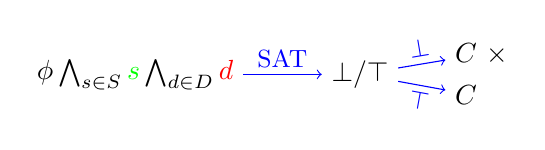
\begin{tikzpicture}
				\tikzset{block/.style={align=center,minimum height=5mm}}
				\node [block] (query) {$\phi \pand \bigwedge_{s \in S} {\color{green}s} \pand \bigwedge_{d \in D} {\color{red}\pnot d}$};
				\node [block, right =10mm of query] (answer) {$\bot/\top$};
				\node [block, above right =-3mm and 6mm of answer] (void) {$C$ $\times$};
				\node [block, below right =-3mm and 6mm of answer] (notvoid) {$C$ \checkmark};
				\path[draw,->,color=blue] (query) edge node[yshift=2mm] {\small SAT} (answer)
							(answer) edge node [yshift=2mm,sloped]{\small $\bot$} (void)
							(answer) edge node [yshift=-2mm,sloped]{\small $\top$} (notvoid);
			\end{tikzpicture}
		}
		\mynextcolumn
		\emph{Cardinality of Partial Configurations (\ssat{})}
		\mydefinition{How Many Products Are Still Configurable for $C$?}{
			\centering
			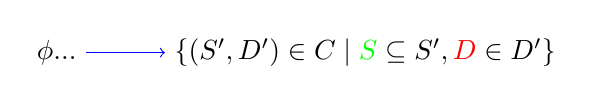
\begin{tikzpicture}
				\tikzset{block/.style={align=center,minimum height=5mm}}
				\node [block] (query) {$\phi \pand ...$};
				\node [block, right =10mm of query] (answer) {$\abs{\{(S', D') \in C \mid {\color{green}S} \subseteq S', {\color{red}D} \in D'\}}$};
				\path[draw,->,color=blue] (query) edge node[yshift=2mm] {\small \ssat{}} (answer);
			\end{tikzpicture}
		}
	\end{mycolumns}
	\begin{mycolumns}[t]
		\myexampletight{}{
			\centering
			{\small\featureDiagram{Root,concrete[X,concrete,optional][Y,concrete,optional]}\\$X \pimplies Y$}

			\cfg{Root}{X} \checkmark
		}
		\mynextcolumn
		\myexampletight{}{
			\centering
			{\small\featureDiagram{Root,concrete[X,concrete,optional][Y,concrete,optional]}\\$X \pimplies Y$}

			\cfg{Root}{X}: 2 products
		}
	\end{mycolumns}
\end{frame}

\subsection{Automated Analyses in FeatureIDE}

\subsubsection*{Feature-Model Editor}

\begin{frame}{\myframetitle}
	\begin{mycolumns}[widths={60,40}]
		\myexampletight{}{
			\pic[width=\textwidth]{featureide-feature-model-editor-waffle}
		}
	\mynextcolumn
		\myexampletight{}{
			\pic[width=\textwidth]{featureide-feature-model-statistics}
		}
	\end{mycolumns}
\end{frame}

\subsubsection*{Configuration Editor}

\begin{frame}{\myframetitle}
	\begin{mycolumns}[widths={60,40}]
		\myexampletight{}{
			\centering
			\pic[width=.27\textwidth]{featureide-configuration-editor-step1}
			$\Rightarrow$
			\pic[width=.63\textwidth]{featureide-configuration-editor-step2}
		}
	\mynextcolumn
		\mynote{Decision Propagation}{
			\begin{itemize}
				\item after each decision (i.e., click) \ldots
				\begin{itemize}
					\item \ldots{} select features that are now \emph{conditionally core}
					\item \ldots{} deselect features that are now \emph{conditionally dead}
				\end{itemize}
				\item this way it is impossible to configure an invalid product
				\item explanations for all propagated decisions
			\end{itemize}
		}
	\end{mycolumns}
\end{frame}

\begin{frame}{Automated Analysis of Feature Models}
	\begin{mycolumns}
		\mydefinition{The Road So Far \ldots}{
			\centering
			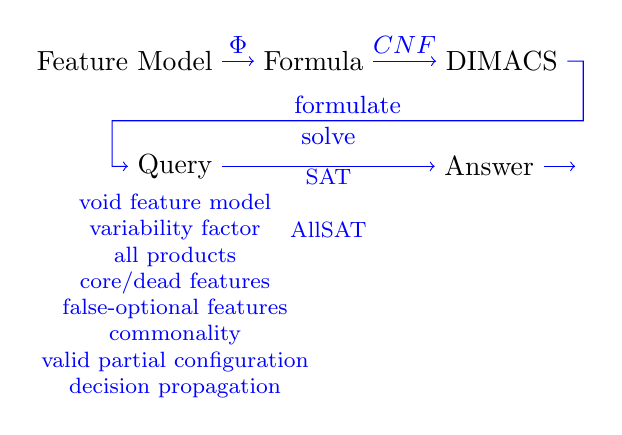
\begin{tikzpicture}
				\tikzset{block/.style={align=center,minimum height=5mm}}
				\node [block] (fm) {Feature Model};
				\node [block, right =4mm of fm] (formula) {Formula};
				\node [block, right =8mm of formula] (cnf) {DIMACS};
				\node [block, below right =8mm and -12mm of fm] (query) {Query};
				\node [block, below =-.5mm of query,align=center,color=blue,font={\footnotesize}] (query2) {void feature model\\variability factor\\all products\\core/dead features\\false-optional features\\commonality\\valid partial configuration\\decision propagation};
				\node [block, right =27mm of query] (answer) {Answer};
				\node [block, right =4mm of answer] (result) {};
				\node [coordinate, below right =5mm and 2mm of cnf] (right) {};
				\node [coordinate, above left =3mm and 2mm of query] (left) {};
				\path[draw,->,color=blue] (fm) edge node[yshift=2mm] {\small $\Phi$} (formula)
							(formula) edge node[yshift=2mm,align=center] {\small $CNF$} (cnf)
							(cnf.east) -| (right) -- node[yshift=2mm] {\small formulate} (left) |- (query)
							(query) edge node[yshift=-2mm,align=center,font={\footnotesize}] {{\small solve}\\[1.5ex]SAT\\\ssat{}\\AllSAT} (answer)
							(answer) edge (result);
			\end{tikzpicture}
		}
	\mynextcolumn
		\mydefinition{\ldots and Beyond}{
			\centering
			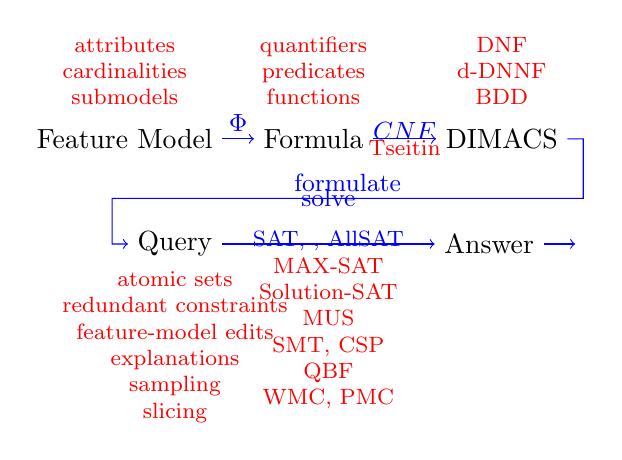
\begin{tikzpicture}
				\tikzset{block/.style={align=center,minimum height=5mm}}
				\node [block,align=center,color=red,font={\footnotesize}] (fm2) {attributes\\cardinalities\\submodels};
				\node [block, below =.5mm of fm2] (fm) {Feature Model};
				\node [block, right =4mm of fm] (formula) {Formula};
				\node [block, above =.5mm of formula,align=center,color=red,font={\footnotesize}] (formula2) {quantifiers\\predicates\\functions};
				\node [block, right =8mm of formula] (cnf) {DIMACS};
				\node [block, above =.5mm of cnf,align=center,color=red,font={\footnotesize}] (cnf2) {DNF\\d-DNNF\\BDD};
				\node [block, below right =8mm and -12mm of fm] (query) {Query};
				\node [block, below =-.5mm of query,align=center,color=red,font={\footnotesize}] (query2) {atomic sets\\redundant constraints\\feature-model edits\\explanations\\sampling\\slicing};
				\node [block, right =27mm of query] (answer) {Answer};
				\node [block, right =4mm of answer] (result) {};
				\node [coordinate, below right =5mm and 2mm of cnf] (right) {};
				\node [coordinate, above left =3mm and 2mm of query] (left) {};
				\path[draw,->,color=blue] (fm) edge node[yshift=2mm] {\small $\Phi$} (formula)
							(formula) edge node[yshift=0mm,align=center] {\small $CNF$\\{\footnotesize\color{red}Tseitin}} (cnf)
							(cnf.east) -| (right) -- node[yshift=2mm] {\small formulate} (left) |- (query)
							(query) edge node[yshift=-7mm,align=center,font={\footnotesize}] {{\small solve}\\[1.5ex]SAT, \ssat{}, AllSAT\\{\color{red}MAX-SAT}\\{\color{red}Solution-SAT}\\{\color{red}MUS}\\{\color{red}SMT, CSP}\\{\color{red}QBF}\\{\color{red}WMC, PMC}} (answer)
							(answer) edge (result);
			\end{tikzpicture}
			\vspace*{-4ex}
			\begin{itemize}
				\item develop new analyses
				\item improve efficiency of existing analyses
				\item investigate correctness and compositionality
			\end{itemize}
		}
	\end{mycolumns}
\end{frame}